\newgeometry{left=4cm, right=4cm,bottom=4cm, top=4cm}
\chapter[Neutral MSSM Higgs Bosons Search...]{Search for neutral MSSM Higgs Bosons in  
$A/h/H \rightarrow \tau^{+}\tau^{-} \rightarrow e \mu + 4\nu$ decays} \label{chap:anal}



 \vspace{0.5cm}

%A search for neutral MSSM Higgs bosons with the ATLAS detector at the
%LHC is presented.  This analysis is based on an integrated luminosity of $20.3 ~fb^{-1}$
%of proton-proton collisions at a center-of-mass energy of 8 TeV. 
%
%The analysis focusses on the decay of neutral Higgs bosons into a pair of tau
%leptons, which subsequently decay to an electron, a muon and four
%neutrinos. Furthermore, 
%
In light of the recent discovery of a Higgs 
boson with mass of $\sim 126$ GeV at LHC~\cite{AHiggsO,CHiggsO}, it remains an open question
whether this new particle is the only missing piece of the electroweak symmetry breaking
sector or whether it is one of several Higgs bosons predicted in some theories 
that go beyond the SM. The most recent measurements \cite{ASpin0,ACouplings,CFermions,CWidth} of its
properties shows this new boson to be, within experimental uncertainties, fully
compatible with the SM Higgs boson. Nevertheles, such a new particle can also still
be accommodated within several theories beyond the 
standard model (BSM), among all of them, Supersymmetry  is a theoretically favoured scenario
as the most predictive framework beyond the Standard Model.

This chapter presents the search for the neutral MSSM Higgs bosons decaying into pairs of tau leptons
in the fully leptonic final state, published in Ref.~\cite{}\footnote{to Sandra: I'll remove this sentence
if Conf note wont be ready in time} as a part of the search for the neutral
MSSM Higgs bosons in all final states of the tau leptons decay. 
The search is based on 20.3 $\text{fb}^{-1}$ of 8 TeV data 
recorded by the ATLAS experiment during 2012 at the Large Hadron Collider.
The chapter is organized as follows: a brief summary of the MSSM Higgs sector 
and an introduction to the analysis strategy is given in Section~\ref{sec:intro},
while the event selection and categorization are described in Section~\ref{sec:selection}. 
In Section~\ref{sec:BackgroundEstimation} the estimation of the background is described and
in Section~\ref{sec:Systematics} methods to evaluate systematic uncertainties are discussed. Finally, 
in section~\ref{sec:result}, an overview of the statistical methods employed along with the corresponding
result of the search are presented.

%There are two approach to explore the Higgs sector:
%one can study the coupling of the Higgs boson with vector
%bosons and fermions, those measure in fact are sensitive to new physics and can determine
%%given the unitarily property of scattering
%%amplitudes for longitudinal vectors and fermions, one can understand 
%if this particle is  fully responsible for
%the generation of all the SM particles masses. 
%Another approach is to directly search for %model dependent
%for additional Higgs es in a well defined model, which is the approach followed in this
%thesis where new neutral bosons are sought within the MSSM (see chapter \ref{}). 
%
%
%%Discovering the mechanism responsible for electroweak
%%symmetry-breaking and the origin of mass for elementary particles has been
%%one of the major goals of the physics program at the Large Hadron
%%Collider~(LHC)~\cite{LHC}.  In the Standard Model (SM) this mechanism
%%requires the existence of a single scalar particle, the Higgs
%%boson~\cite{ENGLERT,HIGGS,HIGGS2,HIGGS3,Guralnik:1964eu}.
%
%%This chapter is divided in three sections:
%%in section~\ref{sec:strategy} an introduction to experimental searches and to the strategy
%of this particular analysis is given, in section~\ref{sec:bkg} is described the core of this thesis
%work, i.e. the detail of the background modeling for this analysis, while in section~\ref{sec:result}
%the result of the search are presented.


\restoregeometry
\clearpage

\section{Introduction } \label{sec:intro}

\subsection{The Higgs Sector in the MSSM}

\begin{figure}[tp]
     \begin{center}

            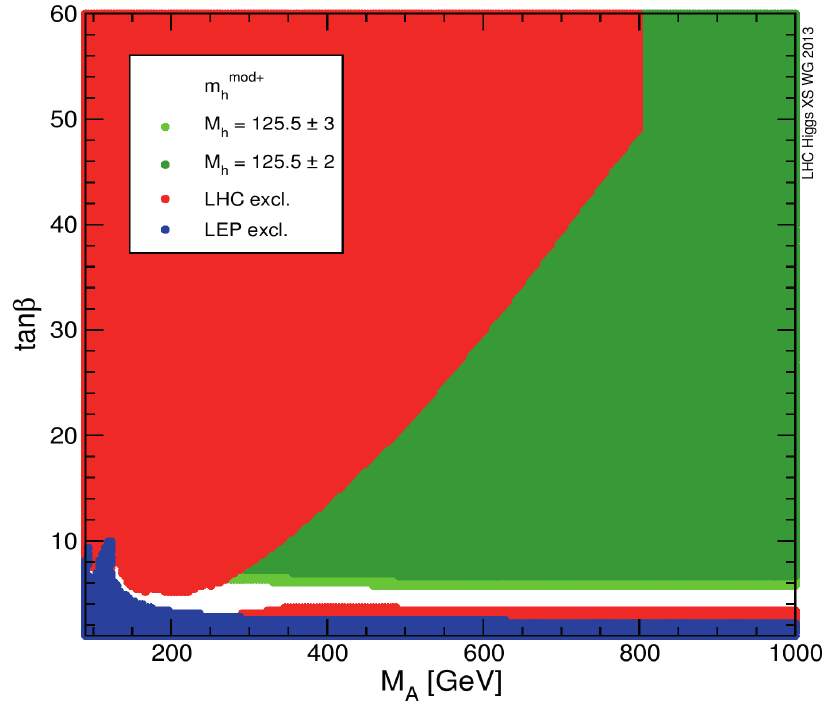
\includegraphics[width=0.6\textwidth]{figure/mh_mod.png}

    \end{center}
    \caption{Excluded and allowed regions of the $m_{A} - \text{tan}\beta$ parameter space for the  $m_{h}^{mod+}$ 
	MSSM benchmark scenario. Excluded regions are determined based on direct Higgs boson searches at LEP 
	(blue) and LHC (red). The two green 
	bands correspond to the parameter regions which are compatible with the assumption that 
	the lightest MSSM Higgs boson, \emph{h}, has a mass respectively of $M_{h} = 125.5 \pm 2$ (dark green) 
	or $125.5 \pm 3$ GeV (light green). For more detail 
	see~\cite{LHCxsec}.}
   \label{fig:mhmod}
\end{figure}

In the Minimal Supersymmetric extension of the Standard Model
(MSSM)~\cite{MSSM1, MSSM2} the Higgs sector is composed of two Higgs
doublets of opposite hyper-charge, resulting in five observable Higgs
bosons:  two of these are neutral and $CP$-even
($h$,$H$), one is neutral and $CP$-odd ($A$) and two are charged
($H^\pm$).  At tree level their properties such as masses, widths and
branching ratios can be predicted in terms of only two parameters,
often chosen to be the mass of the $CP$-odd Higgs boson $m_A$ and
the ratio of the vacuum expectation values of the two Higgs doublets
$\tan\beta$ (for more details see chapter~\ref{chap:theory}).  
The MSSM predicts the existence of a Higgs boson with properties that  
resemble those of a SM Higgs boson in large regions of its parameter space. 
This is usually the case for the lightest Higgs boson, \emph{h}, while the other two, $H$ and $A$, 
tend to be degenerate in mass and decouple from gauge bosons.
%Production and decay mode 
%with vector bosons are forbidden for the CP-odd, $A$ and are suppressed for 
%the CP-even, $H$, Higgs bosons. 
On the other hand, the couplings of the latter two Higgs bosons with down (up) type fermions are enhanced
(suppressed) proportionally to the value of $\tan\beta$, meaning that for large $\tan\beta$
bottom-quark and $\tau$ lepton will play an important role for the Higgs bosons production and its decays. 
 
The two most relevant MSSM Higgs bosons production mechanisms 
at the LHC are gluon fusion, $gg\rightarrow A/H/h$, and 
the production in association with $b$-quarks, $pp \rightarrow b(b)A/h/H$, the latter becoming increasingly 
important for large values of $\tan\beta$. These two are the only production mechanisms
considered in this analysis. 
Assuming there are no decays into supersymmetric particles since these are too heavy, 
the favored neutral MSSM Higgs bosons decay mode  is the decay into a pair of b-quark and antiquark,
$A/h/H \rightarrow b\bar{b}$. This is followed, for the CP-odd $A$ and CP-even $H$ Higgs bosons, 
by the decay into pairs of $\tau$ leptons. Given that it is very difficult to distinguish the former decay 
from the large $b\bar{b}$ background, the decay mode 
$A/h/H \rightarrow \tau^+ \tau^-$  provides the highest sensitivity in the search for neutral MSSM Higgs bosons.

Searches for neutral MSSM Higgs bosons have been performed at
LEP~\cite{LEPLimits}, the
Tevatron~\cite{TevatronLimits1} and the LHC~\cite{CMSLimit, ATLASLimit}. 
In the following the search for the neutral MSSM Higgs bosons  in the final state 
$A/h/H \rightarrow \tau^+ \tau^- \rightarrow e \mu +4\nu$ is presented. 
This search is complementary to the searches in other $\tau^+\tau^-$ final states
characterized by the presence of one or two hadronicaly decaying $\tau$ leptons. Despite of the fact that the 
$\tau\tau$ branching ration in $e \mu +4\nu$ is only 6\%, this decay channel provides a sensitivity 
to the signal comparable to those in other $\tau\tau$ final states, especially for low $m_A$ values. 
This is mainly due to the high transverse momentum treshold at the trigger level for  hadronicaly decaying $\tau$ leptons.

As it is impractical for an experimental  search to explore the full parameter space of the MSSM, 
which has many free paramers, several benchmark scenarios are  
introduced by fixing all except $m_A$ and $\tan\beta$ parameters to values typical for most interesting 
physics cases.
With the recent Higgs boson discovery, benchmark scenarios of the MSSM have been updated to 
accommodate for  new experimental constraints. 
As an example, Figure~\ref{fig:mhmod} shows the currently excluded and allowed regions of the MSSM parameter space
for the  $m_{h}^{mod+}$ updated benchmark scenario. In this scenario a large region of the $m_{A} - \text{tan}\beta$
parameter space is compatible with the assumption that the observed Higgs boson correspond to the supersymmetric
SM-like Higgs boson, $h$. A large part of this parameter space is still experimentally unexplored,
this is a strong motivation to pursue the search for additional neutral MSSM Higgs bosons.


\subsection{Signal and Background Processes}
Signal events, in which the neutral MSSM Higgs bosons decays trough 
$A/h/H \rightarrow \tau^+ \tau^- \rightarrow e \mu +4\nu$, are characterized 
by the presence of one electron and one muon of opposite charge, these are isolated and with 
relatively high transverse momentum, additionally, four neutrinos contribute to the missing transverse energy of the event. 
Figure~\ref{fig:feyndiagSignal} shows leading order Feynman diagram for the two signal production mode considered,
gluon-gluon fusion and b-associated production.
The production modes also contributes to the characterization of the signal topology: the presence or the absence 
of b-jet in the final state is expected in case of  b-associated or gluon-gluon fusion production mode, respectively.

\begin{figure}[tp]
     \begin{center}

          %  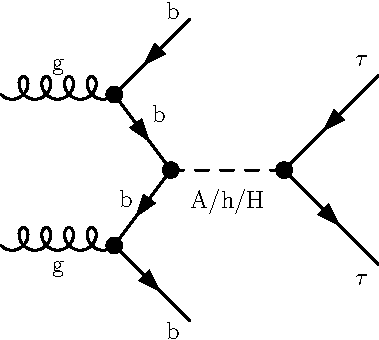
\includegraphics[width=0.3\textwidth]{feyn_diagrams/diagrams/bbA.pdf}\hspace{1cm}
          %  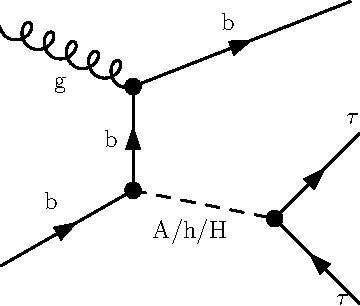
\includegraphics[width=0.3\textwidth]{feyn_diagrams/diagrams/bbA2.pdf}\hspace{1cm}
          %  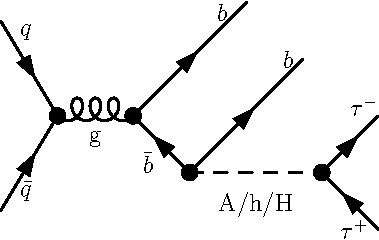
\includegraphics[width=0.3\textwidth]{feyn_diagrams/diagrams/bbA3.pdf}\\
          %  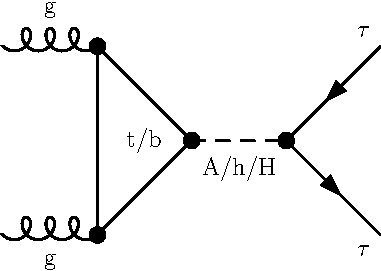
\includegraphics[width=0.3\textwidth]{feyn_diagrams/diagrams/ggH.pdf}

    \end{center}
    \caption{To Sandra: the diagrams are will be updated asap.}    
	
   \label{fig:feyndiagSignal}
\end{figure}


The signal topology  just described is common to several other processes, which unfortunately, 
have higher cross section than the sought signal.
The dominant backgrounds for this search are the production of  $Z/\gamma^* \rightarrow \tau^+ \tau^- $
either via Drell-Yan process or in association with jets and the top quark production ($t\bar{t}$ and single top production is intended). 
Additional significant backgrounds are  dibosons production 
($WW$, $WZ$, $ZZ$) and  events with non-prompt leptons coming solely from hadron decay (QCD multi-jet).
Vector bosons production like  $\Wlnu$ or $\Zll$ in association with jets (with $\ell$ here meaning either $e$ or $\mu$) 
are also considered, however these processes have a limited impact. Figure~\ref{fig:feyndiagBack} shows few relevant examples of 
leading order Feynman diagrams for the dominant background processes.
The production cross sections times the relevant branching fraction for signal and backgrounds are summarized in
Table~\ref{tab:MCxsec}. 
%The $W/Z$ and $b\bar{b}A/H/h$ production cross sections 
%are calculated to NNLO. The one for $\ttbar$, single top and dibosons cross sections are calculated at NLO.
%Finally, the direct $gg\rightarrow A/H/h$ signal cross sections 
%are calculated at NNLO and NLO for the top loop and the bottom loop respectively.
%

\begin{figure}[tp]
     \begin{center}

          %  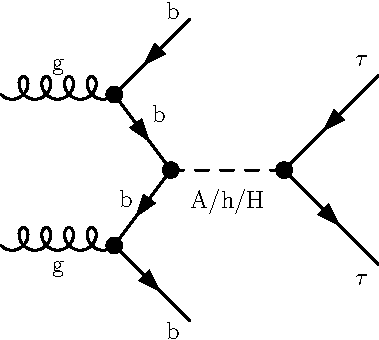
\includegraphics[width=0.3\textwidth]{feyn_diagrams/diagrams/bbA.pdf}\hspace{1cm}
          %  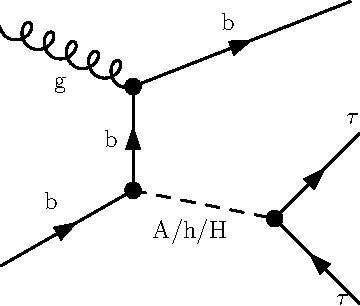
\includegraphics[width=0.3\textwidth]{feyn_diagrams/diagrams/bbA2.pdf}\hspace{1cm}
          %  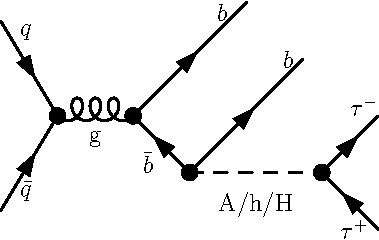
\includegraphics[width=0.3\textwidth]{feyn_diagrams/diagrams/bbA3.pdf}\\
          %  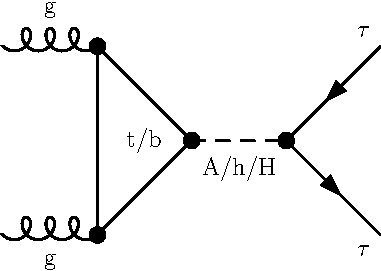
\includegraphics[width=0.3\textwidth]{feyn_diagrams/diagrams/ggH.pdf}

    \end{center}
    \caption{To Sandra: the diagrams are will be updated asap.}    
	
   \label{fig:feyndiagBack}
\end{figure}


%The values of the steering parameters used for the HERWIG, JIMMY and PYTHIA
%generators are described in Ref.~\cite{ATLASMC09Tune}.

\begin{table}[tp]
\begin{center}
%\begin{footnotesize}
\begin{small}
\begin{tabular}{lr}
\hline \hline
Process                                                                 & Cross-section~(pb) [$\times$ BR] \\ [1pt]
\hline
\multicolumn{2}{c}{Signal ($m_A=150$~GeV, $\tan\beta=20$, $m_{h}^{max}$ scenario) }  \\ [1pt]

$gg\rightarrow A/h/H \rightarrow\tau\tau \rightarrow e\mu+ 4\nu)$                 &  $0.12 / 0.09 / 0.13$ \\
$pp \rightarrow b\bar{b}A/h/H \rightarrow \tau\tau \rightarrow e\mu + 4\nu)$       & $ 0.29 /0.03 / 0.25   $ \\[1pt]
\hline
\multicolumn{2}{c}{Backgrounds} \\[1pt]
$W\rightarrow \ell$+jets                           & 12.22$\times 10^3$ \\
$Z/\gamma^{*}\rightarrow \ell\ell$+jets       & 5.5$\times 10^3$ \\
$t\bar{t} \rightarrow \ell \ell + X$                                                              & 137.3 \\
Single top ($t$, $s$ and $Wt$ channels) $\rightarrow \ell + X$               & 28.4, 1.8, 22.4 \\
Dibosons WW, WZ and ZZ  $\rightarrow \ell + X$                                          & 20.6, 6.8, 1.55 \\ [1pt]
\hline 
\hline
\end{tabular}
\end{small}
\caption{The cross sections multiplied by the relevant branching ratios~(BR) for signal and the considered
backgrounds. the symbol $\ell$ stands for $\ell= (e, \mu, \tau)$. 
Signal cross sections are calculated for the $m_{h}^{max}$ scenario shown for
 $m_A=150$~GeV and $\tan\beta=20$, in this case  $m_H=151$~GeV and $m_h=129$~GeV.}
 \label{tab:MCxsec}

\end{center}
\end{table}


\subsection{Analysis Strategy} \label{sec:strategy}


In this thesis a search for the MSSM 
$A/h/H \rightarrow \tau^+ \tau^- \rightarrow e \mu +4\nu$ is presented. The $e-\mu$ final state 
is chosen out of the three possible fully 
leptonic final state of a $\tau^+ \tau^-$ resonance,
the choice is motivated by the fact that it represent the 50\% of the the fully leptonic final states and 
because the $e-e$ and $\mu-\mu$ case are not expected to bring significant sensitivity, in fact in these cases, large background
contribution are expected not only from $\Ztautau$ but also from $\Zee$ and $\Zmumu$,  respectively.

Candidate events are selected based on the topological properties of the Higgs boson production
and decay, the events are required to present one electron and one muon, isolated and of opposite charge.
The set of events is divided in two orthogonal category which are optimized separately
for the two different production mode considered. In the gluon-gluon fusion category (also called \emph{b-vetoed} category),
the absence of a b-tagged jet is required, the main background in this category is $\Ztautau$. 
In contrast, the presence of a b-tagged jet is required for b-associated production category (also called 
\emph{b-tagged} category), the request of a b-jet suppress the $\Ztautau$ background, $\ttbar$ and single top production
are then the main backgrounds in this category.

The $A/h/H \rightarrow\tau\tau \rightarrow e\mu+ 4\nu$ search is performed in the MSSM $m_h^{max}$ benchmark scenario
scanning the $m_A - \tan\beta$ plane in the ranges $90 \leq m_A \leq 300$ GeV and $5 < \tan\beta < 60$,
the signal prediction for the event yield and kinematical distributions is evaluated by simulation.

The dominant $\Ztautau$ background is estimated from data via a signal-depleted control sample.
The  QCD multi-jet background contribution is also estimated from data since it represent a challenge for MC simulation.  
The estimation of the contribution of  all the other backgrounds is obtained by means of MC simulation.
The background model predictions are validated using different signal-depleted control data samples, 
good agreement is found.

The systematics uncertainties taken into account for simulated signal and backgrounds arise from uncertainties on  
cross section calculations and on the modeling of the detector response. For backgrounds that are estimated from data,
specific uncertainty are evaluated considering the possible uncertainties of the estimation methods.


The final statistical interpretation of the data is based on the 
comparison of the observed invariant mass distributions with the expected background and signal-plus-background
predictions. Exclusion limits are set by means of a binned likelihood ratio
test statistic. The limits are interpreted  in the MSSM $m_{h}^{max}$ scenario and evaluated as a function
of $m_A$ and $\tan\beta$. Furthermore, the limits are interpreted, in a less model depended
way, in terms of the cross section for the production of a generic Higgs boson, $\phi$, of mass  $m_\phi$, 
via the production mode $pp \rightarrow b\bar{b}\phi$ and $gg \rightarrow \phi$.


 

%neutral MSSM Higgs bosons with the ATLAS experiment at CERN is
%presented, using proton-proton collisions at center-of-mass energy of
%8~TeV, with a recorded integrated luminosity of
%$20.3 \ifb$.



\subsection{Data and Simulated Event Samples}
\label{sec:sample}
\subsubsection{Data Sample}

The  presented result  are based on proton-proton collision data
collected at the LHC during 2012 at a center-of-mass energy of $\sqrt{s}=8$~TeV,
corresponding to an integrated luminosity of 20.3 fb$^{-1}$.
The events used in this analysis are recorded using a combination of a
single electron and combined electron-muon triggers. Only recorded events 
in which all the relevant components of the ATLAS detector were
fully operational are considered.
Additional data quality requirements are applied to the events according to~\cite{ATLASCLEANING},
these requirements assures the rejection of  events with data corruption due to the LAr and Tile calorimeters and
with jet activity in known noisy calorimeter regions. 




\subsubsection{Signal Samples}
%Both the signal and background process modelled by Monte Carlo (MC)
%simulation were produced within the ATLAS MC12a production campaign.
%The generators used for the different processes are described below.
Signal production via the gluon fusion process, $gg\rightarrow A/H/h$,
was simulated with POWHEG~\cite{POWHEG} and the associated
$b\bar{b}A/H/h$ production with SHERPA~\cite{SHERPA}.  The
pseudo scalar Higgs boson samples were generated in the mass range from
90~GeV to 300~GeV and at $\tan\beta = 20$, the same kinematics
are assumed for $A/h/H$ Higgs bosons decay products and at other
$\tan\beta$ values, appropriate re weighting is applied according to the
different cross-sections. The $m_h^{\mathrm{max}}$ MSSM benchmark
scenario is assumed.


\subsubsection{Background Samples}
The production of $W$ and $Z/\gamma^*$ bosons in association with jets
was simulated with the ALPGEN~\cite{Alpgen} generator. 
%This employs
%the MLM matching scheme~\cite{MLM} between the hard process,
%calculated with leading-order matrix elements for up to five jets, and
%the parton shower.  
The $t\bar{t}$ process was generated using the POWHEG generator. The single-top (s-channel, $Wt$)
processes were generated using MC@NLO~\cite{MCatNLO}, while single-top
(t-channel) processes were generated with AcerMC~\cite{AcerMC}.  The
production of dibosons~($WW$, $WZ$, $ZZ$) were generated with
HERWIG~\cite{Herwig}.  For all ALPGEN and MC@NLO samples described
above, the parton shower and hadronisation were simulated with HERWIG
and the activity of the underlying event with JIMMY~\cite{JIMMY}.
%The loop-induced $gg\rightarrow WW$ processes were generated using gg2WW~\cite{GG2WW}.  We are not using it Xsec very small
Different parton density functions (PDFs) sets are used depending on
the generator: CTEQ6L1~\cite{CTEQ6} is used by ALPGEN and AcerMC while
CT10~\cite{CT10} is used by SHERPA, POWHEG and MC@NLO. 

TAUOLA~\cite{TAUOLA} and PHOTOS~\cite{PHOTOS} are used to model the
tau lepton decay and additional photon radiation from charged leptons
in the leading-log approximation, respectively.

The ATLAS detector response is simulated for all the MC samples using GEANT4~\cite{Geant4,ATLASSIM},
the physics object reconstruction is performed with the same software as for data described in chapter~\ref{chap:obj}.
The effects of the simultaneous recording of several events from the
same or neighboring bunch crossings (pile-up) are considered in the
simulation. 



\section{Event Selections and Categorization}\label{sec:selection}


\subsection{The ``Common'' Selections}\label{sec:presel}

According to the signal events characteristics, each event either data and MC should satisfy
the following selection criteria, these selections are shared by both analysis category and therefore 
referred in the following as ``common selections'':


\begin{enumerate}[label=(\roman*)]
\item A trigger selection, requiring the presence of an electron with $\pt > 24$ GeV, or alternativaley,
	an electron with  $\pt > 12$ GeV togheter with a muon with  $\pt > 8$ GeV. 

\item At least one reconstructed vertex with more that three associated tracks. This selection is aimed to 
	reject background from cosmic muons.

\item Exactly one reconstructed ``Tight'' electron with $|\eta| < 1.37 $ or $1.52 < |\eta| < 2.47$.
	The electron  should have $\pt > $ 15 or 25~GeV depending on the trigger that selected the event. 

\item Exactly one ``Combined'' muon with $|\eta| < 2.5$ and  $\pt > $ 10~GeV.

\item The electron should be isolated with $E_T^{cone}/\pt < 0.08$ and $P_T^{cone}/\pt < 0.06$ .

\item The muon should be isolated with  $E_T^{cone}/\pt < 0.04$ and $P_T^{cone}/\pt <  0.06$ 

\item Muon and electron should be of opposite charge.

\item Overlap removal between electron, muon, $\tau_h$ and jets is performed.

\item The events is rejected if at least one hadronic $\tau$ decay is found with $\pt > $ 15 GeV.

\item The invariant mass of the sum of the electron and muon 4-vectors should be greather than 30 GeV.

\end{enumerate}
For details about the definition of physics object used above and their quality requirements  refer to chapter~\ref{chap:obj}.
 
The two analysis category, \emph{b-tagged} and \emph{b-vetoed}, are defined adding on top of the common selections 
the request of exactly one b-tagged jet or the absence of b-tagged jet in the event respectively. To be 
\emph{taggable} a jet should have $\pt > 20$ GeV, $|\eta| < 2.5$ and $\text{JVF} > 0.5$.
A jet is considered tagged if passes the selection of the $MV1$ algorithm at 70\% of efficiency for b-quark, 
$\epsilon_b^{\ttbar}$. Further selection
are applied to each category and optimized separately, these additional selection are described in the following.

\subsection{b-vetoed Category}\label{sec:veto}
%\subsection{Selections}

The final state of Higgs decaying into tau pair coincide with the one from  $\Ztautau$  process, this is then an irreducible 
background for this category. Exploiting the different kinematics of the Higgs decay with respect to 
other backgrounds is possible to disentangle
between them. In the Higgs decaying into $\tau^{+} \tau^{-} \rightarrow e ~ \mu + 4\nu$ the taus are highly boosted
and this feature is transferred to the final state leptons, their kinematics then result to be  significantly different 
with respect to process like diboson or $\ttbar$. A first difference is that  $e$ and $\mu$ from the Higgs decay 
will be more likely "back-to-back",
as it is shown in Figure~\ref{dphi} where the angle between the leptons in the transverse plane 
$\Delta\phi_{e,\mu} = |\phi_{e} - \phi_{\mu}|$ 
is reported.  Furthermore the neutrinos will be more likely collinear with the charged leptons:
this feature can be matematically seen as the sum of scalar product between missing energy and the leptons four-vectors in the
transverse plane, if the vectors are normalised to unit versors then what remains is a relation only between angles:
$$ \hat{E}_{T}^{miss} \cdot ( \hat{P}_{T}^{\mu} + \hat{P}_{T}^{e} ) = cos(\Delta\phi_{E_{T},\mu}) 
+ cos(\Delta\phi_{E_{T},e}) = \sum_\ell cos(\Delta\phi_{E_{T},\ell}) $$
collinearity implies this sum to be equal to zero as it is shown in Figure~\ref{sumcosphi}. 
These two feature can be used to distinguish between $e-\mu$ and $\met$ coming from decay of highly 
boosted and back-to-back object and the one coming from W decays in top or in dibosons backgrounds,
in which the leptons are not necessarily back-to-back and the neutrinos not collinear with them.
In b-vetoed category these two variables are sufficient to suppress contribution from dibosons,
no other selection is applied in this category because it has been shown to not bring significant improvement.
The actual selection employed in this category are shown in Table~\ref{tab:sel}, while in Table~\ref{tab:eventsel:bveto}
the prediction for the number of background and signal events that survises at 
each selection stage of this category is reported.


\begin{table}[t]
  \begin{center}
   %\begin{footnotesize}	
    \begin{tabular}{p{4cm}c}
      \hline \hline
      Category & Selection \\ [3pt]
      \hline
%      Common Selection 	&  Trigger \\
%	&	At least one reconstructed vertex with $> 3 $ tracks \\
%	& 	Exactly one tight isolated electron with $\pt > 15 $ or 25 GeV  \\
%	&	Exactly one Combined isolated muon with  $\pt > 10$ GeV \\
%	& 	Opposite charge between electron and muon \\ 
%	&	Overlap removal\\
%	&	Tau Veto \\
%	&	$M_{e-\mu} > 30$ GeV \\
%      \hline
      b-vetoed & Exactly zero b-tagged taggable jets \\	
      & $\Delta\phi(e-\mu)>1.6$ \\
      & $\sum\cos\Delta\phi > -0.4$ \\[5pt]
      \hline
      b-tagged & Exactly one b-tagged taggable jet \\
      & $\Delta\phi(e-\mu)>2$ \\
      & $\sum\cos\Delta\phi > -0.2$ \\
      & $ H_T < 100$ GeV \\
      & $P_{T\mu} + P_{Te} + \met < 100$ GeV \\[3pt]
      \hline \hline
    \end{tabular}
    \caption{Summary of the dedicated b-tagged and b-vetoed category selections that are employed after the common selections.}
    \label{tab:sel}
  %\end{footnotesize}
  \end{center}
\end{table}

\subsection{b-tagged Category}\label{sec:tag}
In the b-tagged category the situation is different, 
the  request of a b-jet enhance backgrounds with b-jet activity as top and single top production.
In this category selection on $\Delta\phi(e-\mu)$ and $\sum\cos\Delta\phi$  are employed as described for b-vetoed,
since these selections are effective in reducing top and diboson backgrounds. In addition further selection exclusive of this category
are employed  and are described below.

Given the relatively low jet activity of Higgs events (also in the case of b-associated production), 
it is possible to separate them from
top production which instead is very likely to have two or more highly enegetic jets in the event.
Little jet activity is achieved by requesting the sum of the jets $\pt$ in the event to be small, this variable is called $\Ht$
and is shown in Figure~\ref{Ht}. The jets used for the calculation of $H_T$ should have $\pt > 30 $ GeV, $|\eta| < 4.5$  and
$\text{JVF} > 0.5 $ (when applicable).

Another feature that distinguish top pair production from Higgs is the higher invariant mass of the former final state
(the highest Higgs mass considered for this search is 300 GeV),
in the transverse plane all the leptons will tend to have a higher momentum, the sum of electron and muon \pt and \met is then used as
a discriminating variable. Figure~\ref{sumlepPt} shows the distribution of this last analysis variable.

The above described variables defines the b-tagged category, in table~\ref{tab:sel} a summary of all the employed selection 
variables with their optimized cut values is shown. In Table~\ref{tab:eventsel:btag}
the prediction for the number of background and signal events that survises at 
each selection stage of this category is reported.


\begin{figure}[p]
     \begin{center}
     \subfigure[]{		
            \includegraphics[page=11,width=0.47\textwidth]{figure/std_plots_presel.pdf}
	    \label{dphi}	
     }	
     \subfigure[]{		
            \includegraphics[page=12,width=0.47\textwidth]{figure/std_plots_presel.pdf}
	    \label{sumcosphi}	
     }	
     \subfigure[]{		
            \includegraphics[page=9,width=0.47\textwidth]{figure/std_plots_presel.pdf}
	    \label{Ht}	
     }	
     \subfigure[]{		
            \includegraphics[page=10,width=0.47\textwidth]{figure/std_plots_presel.pdf}
	    \label{sumlepPt}	
     }	

    \end{center}
    \caption{Distribution of analysis variable after the selections common to both category, a comparison of the prediction
	   of background model prediction and data is made showing good agreement.  The yellow band represents the total
		systematic uncertainty for the background model prediction.}
   \label{fig:selections}
\end{figure}




\subsection{Mass Reconstruction with MMC Technique}\label{sec:mmc}

Acurate invariant mass reconstuction of a di-$\tau$ resonace is a challenging task
due to the presence of neutrinos from the $\tau$ leptons decay. 
In case of leptonic decay of both $\tau$ leptons a pair of neutrinos for each
of them are involved in the final state,  the system presents then eight uknowns, which corresponds to the four-momentum of the neutrinos pairs.
Four additional kinematic constraint are set by the following equations:
%There are four additional constraint 
%which come from the measurement of \MET and from the fact that each single decay should have invariant mass equal to the tau mass:
\begin{equation} \label{eq:MMC}
\begin{split}
%\begin{align}
%\begin{gather*}  
&\vec{E}_T^{miss} = \vec{P}_{T}^{mis_{1}} +  \vec{P}_{T}^{mis_2} \\
&M_{\tau_{i}}^2 = m^2_{mis_{i}} + m^2_{vis_{i}} + 2 \mathbf{P}_{vis_i} \cdot \mathbf{P}_{mis_i} \\
%\end{align}
%\end{gather*}
\end{split}
\end{equation}
where the index \emph{i} runs over the two $\tau$ leptons of the event and assumes the values of 1 or 2. 
$\vec{P}_{T}^{mis_{i}}$, $m_{mis_{i}}$ and $\mathbf{P}_{mis_{i}}$ are respectively the transverse momentum, the invariant mass and 
the four momentum of the pair of neutrinos related to the  $\tau$ lepton decay \emph{i} with mass $M_{\tau}$, the subscript \emph{vis} indicates instead 
quantities related to the charged lepton from  $\tau$ lepton decay. The system has still four degrees of freedom,
%$m^2_{miss}$, therefore there are still four degrees of freedom in the system.
several approximation are possible to further constraint the momentum carried by neutrinos,
for example assuming them collinear to the electron or muon from $\tau$ lepton decay, however those approximation 
suffers of mass resolution limitations.

\begin{table}[tp]
  \centering
   \begin{footnotesize}	
  \begin{tabular}{ccccc}
    \hline\hline
	&	Common Selections			&	n(b-jet)=0			&	$\Delta\phi(e-\mu)>1.6$			&	$\sum\cos\Delta\phi > -0.4$ 		\\	
    \hline
   \hline
Data	&	125886			&	89155			&	-			&	-				-			\\
Multi-jet	&	6693	$\pm$	456	&	6357	$\pm$	461	&	5322	$\pm$	438	&	4137	$\pm$	339	\\
\Zll 	&	569	$\pm$	48	&	564	$\pm$	48	&	516	$\pm$	47	&	434	$\pm$	44		\\
\Wlnu	&	1625	$\pm$	155	&	1604	$\pm$	155	&	1145	$\pm$	125	&	714	$\pm$	101		\\
Dibosons	&	9338	$\pm$	48	&	9235	$\pm$	48	&	7358	$\pm$	43	&	4002	$\pm$	31		\\
\ttbar	&	40632	$\pm$	106	&	7707	$\pm$	46	&	5044	$\pm$	37	&	3416	$\pm$	31		\\
Single Top	&	4449	$\pm$	44	&	1664	$\pm$	27	&	1124	$\pm$	22	&	682	$\pm$	18	\\
\Ztautau	&	61503	$\pm$	68	&	60440	$\pm$	67	&	58078	$\pm$	65	&	55303	$\pm$	64	\\
Signal	&				&				&	-			&	-						\\
    \hline
  \end{tabular}
  \caption{Number of data and background events in the b-vetoed channel.}
  \label{tab:eventsel:bveto}
   \end{footnotesize}	
\end{table}

\begin{table}[t]
  \centering
   \begin{footnotesize}	
  \begin{tabular}{cccccccc}
    \hline\hline
	& 	n(b-jet)=1			&	$\Delta\phi$&	$\sum\cos\Delta\phi$			&	$P_{T\mu} + P_{Te} + \met$&	$ H_T$	\\
   \hline
Data	&	23352			&	-			&	-			&	-			&	-						\\
Multi-jet	330	$\pm$	40	&	208	$\pm$	27	&	135	$\pm$	22	&	114	$\pm$	17	&	100	$\pm$	15	\\
\Zll 	&	5.2	$\pm$	1.8	&	2.3	$\pm$	1.1	&	2.3	$\pm$	1.1	&	1.7	$\pm$	1.0	&	0.9	$\pm$	0.8		\\
\Wlnu	&	20	$\pm$	6	&	15	$\pm$	6	&	13	$\pm$	6	&	10	$\pm$	6	&	10	$\pm$	6		\\
Dibosons	&	99	$\pm$	5	&	63	$\pm$	4	&	36.4	$\pm$	3.0	&	14.8	$\pm$	1.8	&	13.3	$\pm$	1.8		\\
\ttbar	&	19810	$\pm$	70	&	9680	$\pm$	50	&	6450	$\pm$	50	&	808	$\pm$	15	&	350	$\pm$	10		\\
Single Top &	2456	$\pm$	33	&	1223	$\pm$	23	&	784	$\pm$	18	&	122	$\pm$	7	&	99	$\pm$	7		\\
\Ztautau &	952	$\pm$	9	&	625	$\pm$	7	&	540	$\pm$	7	&	482	$\pm$	6	&	421	$\pm$	6		\\
Signal		&				&	-			&	-			&	-			&	-						\\
    \hline
    \hline
  \end{tabular}
  \caption{Number of data and background events in the b-tagged channel.}
  \label{tab:eventsel:btag}
   \end{footnotesize}	
\end{table}

In this analysis, the so-called "Missing Mass Calculator" (MMC) algorithm
is used to calculate the most likely di-$\tau$ system invariant mass given the event topology, %event kinematics
the implementation of the method in this search is based on~\cite{MMC}. 
The concept of the MMC is to solve equation~\ref{eq:MMC} assigning values to the yet undetermined variables, performing a 
``scan'' over a four dimensional parameter space. The four independent  variables are chosen 
to be $ m^2_{mis_{i}}$ and $cos\theta^*_i$ , the latter defined
as the angle between the charged lepton from the $\tau$ lepton decay and the boost direction of the $\tau$ lepton. 
The di-$\tau$ invariant mass of the event can be calculated for each given point of the parameter space that solves equations~\ref{eq:MMC},
however, the solutions are not all equally likely and  the probability of a given $\tau$ decay configuration can be predicted by means
of simulation (PYTHIA supplemented with TAUOLA package is used). Each point in the parameter space, corresponding
to a particular di-$\tau$ invariant mass, is then weighted by its probability to occur. 
The estimator for the final discriminant, the mass of the di-tau system \mmc, 
is the maximum of the weighted invariant mass distribution calculated for the scanned points.

The missing energy plays an important role in the MMC method and  its resolution has an impact on the calculation
of the invariant mass. To improve $\met$ resolution, a scan over a six dimensional parameter space is performed 
in a similar way as described above, in this case however, $\vec{E}_T^{miss}$ is also considered unknown and a scan 
is performed on it assigning values  according to its uncertainty. 
The probability of each solution is calculated and the final missing transverse
energy is given by the weighted mean of the scanned points. 

The final procedure consist in obtaining first an estimate for $\met$ by means of a six dimensional scan over the solution of equations~\ref{eq:MMC},
successively a four dimensional scan is performed fixing $\met$ to the updated value and calculating the most likely invariant mass 
of the di-$\tau$ system.
Figure~\ref{fig:mass} shows the final state invariant mass distribution calculated with  \mmc 
discriminating variable, the distribution is shown after the common selection and after the full selection
of both category. 

 
%Accurate invariant mass reconstruction of a di-tau system is a challenging task due to the escaping neutrinos.
%In this analysis, with four neutrinos in the final state, the number of unknown largely exceed the number of constraints,
%several approximation are possible to further constraint the neutrinos, for example assuming them collinear to the 
%other leptons from tau decay, however those approximation suffers of limitations. 

%In this analysis we use the so called missing mass calculator (MMC)~\cite{MMC}
%technique for the calculation of the di-tau system invariant mass. This technique employs additional 
%information from the well known tau decay to constraint the system, this is achieved by minimizing a likelihood function 
%defined in the kinematically allowed phase space region, the result is a more precise measurement of the di-tau 
%system invariant mass and a considerable improvement in resolution. The invariant mass distribution 
%calculated with the MMC technique is referred in the following as $\mmc$ and is used as discriminating 
%variable in the limits setting.

\begin{figure}[p]
     \begin{center}
     
     \subfigure[]{		
            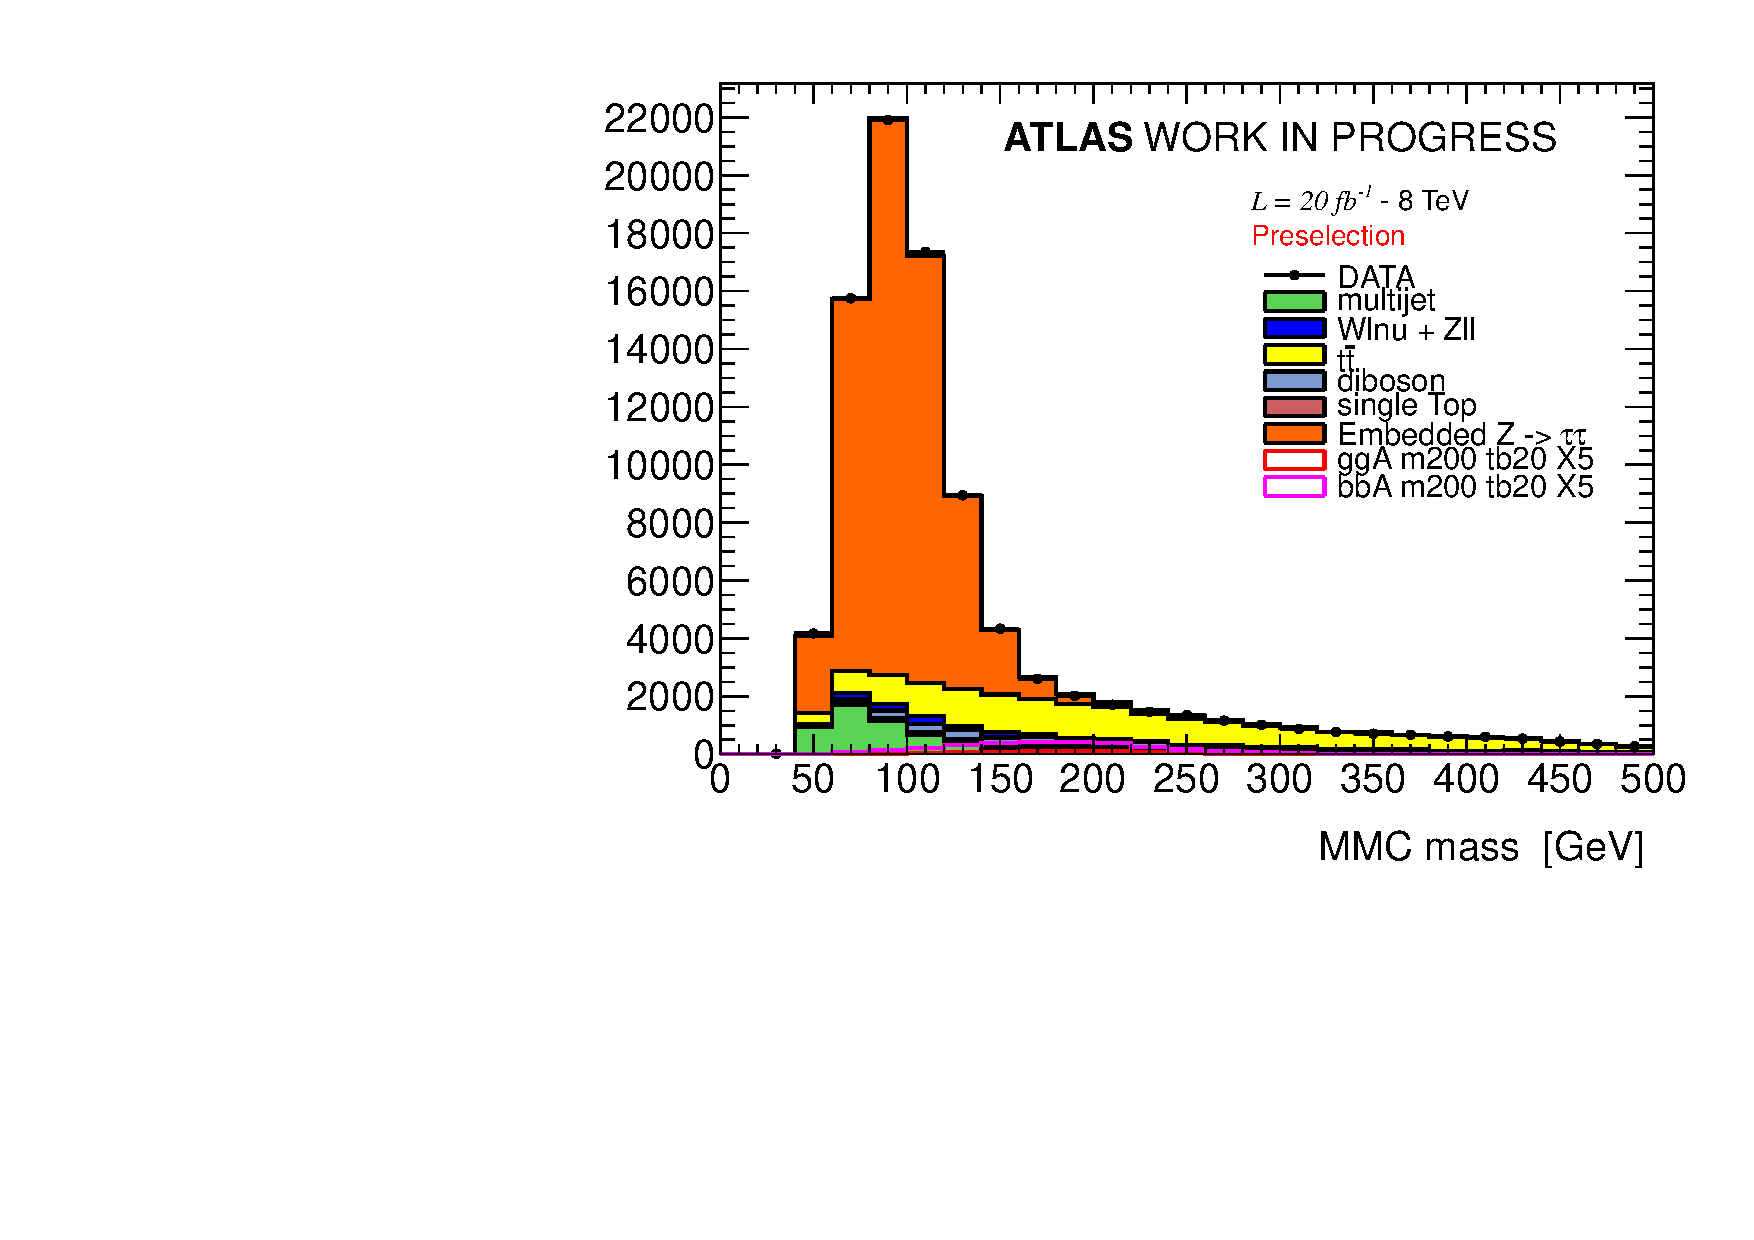
\includegraphics[page=1,width=0.6\textwidth]{figure/std_plots_mass.pdf}
	    \label{presel}	
    	%\caption{\footnotesize common selections.}
     }\\	

%     \subfigure[]{		
%            \includegraphics[page=3,width=0.47\textwidth]{figure/std_plots_mass.pdf}
%	    \label{veto}	
%    	%\caption{\footnotesize b-vetoed.}
%     }	
%     \subfigure[]{		
%            \includegraphics[page=2,width=0.47\textwidth]{figure/std_plots_mass.pdf}
%	    \label{tag}	
%    	%\caption{\footnotesize b-tagged.}
%     }	
     \subfigure[]{		
            \includegraphics[page=7,width=0.6\textwidth]{figure/std_plots_mass.pdf}
	    \label{fullveto}	
    	%\caption{\footnotesize full b-vetoed.}
     }	
%     \subfigure[]{		
%            \includegraphics[page=7,width=0.47\textwidth]{figure/std_plots_mass.pdf}
%	    \label{btagphi}	
    	%\caption{\footnotesize b-tagged + $\Delta\phi$ + $\sum_\ell cos(\Delta\phi_{E_{T},\ell})$.}
%     }
     
     \subfigure[]{		
            \includegraphics[page=6,width=0.6\textwidth]{figure/std_plots_mass.pdf}
	    \label{fullbtag}	
    	%\caption{\footnotesize full b-tagged.}
     }
    \end{center}
     	

    \caption{\footnotesize Distribution of the \mmc for different cuts stage, see text. Left column corresponds to b-tagged category, right column to b-vetoed.}
   \label{fig:mass}
\end{figure}

